\section{BGPmon: Deploying Your Own Monitors}
\label{sec:mesh}

\begin{figure}
\centering
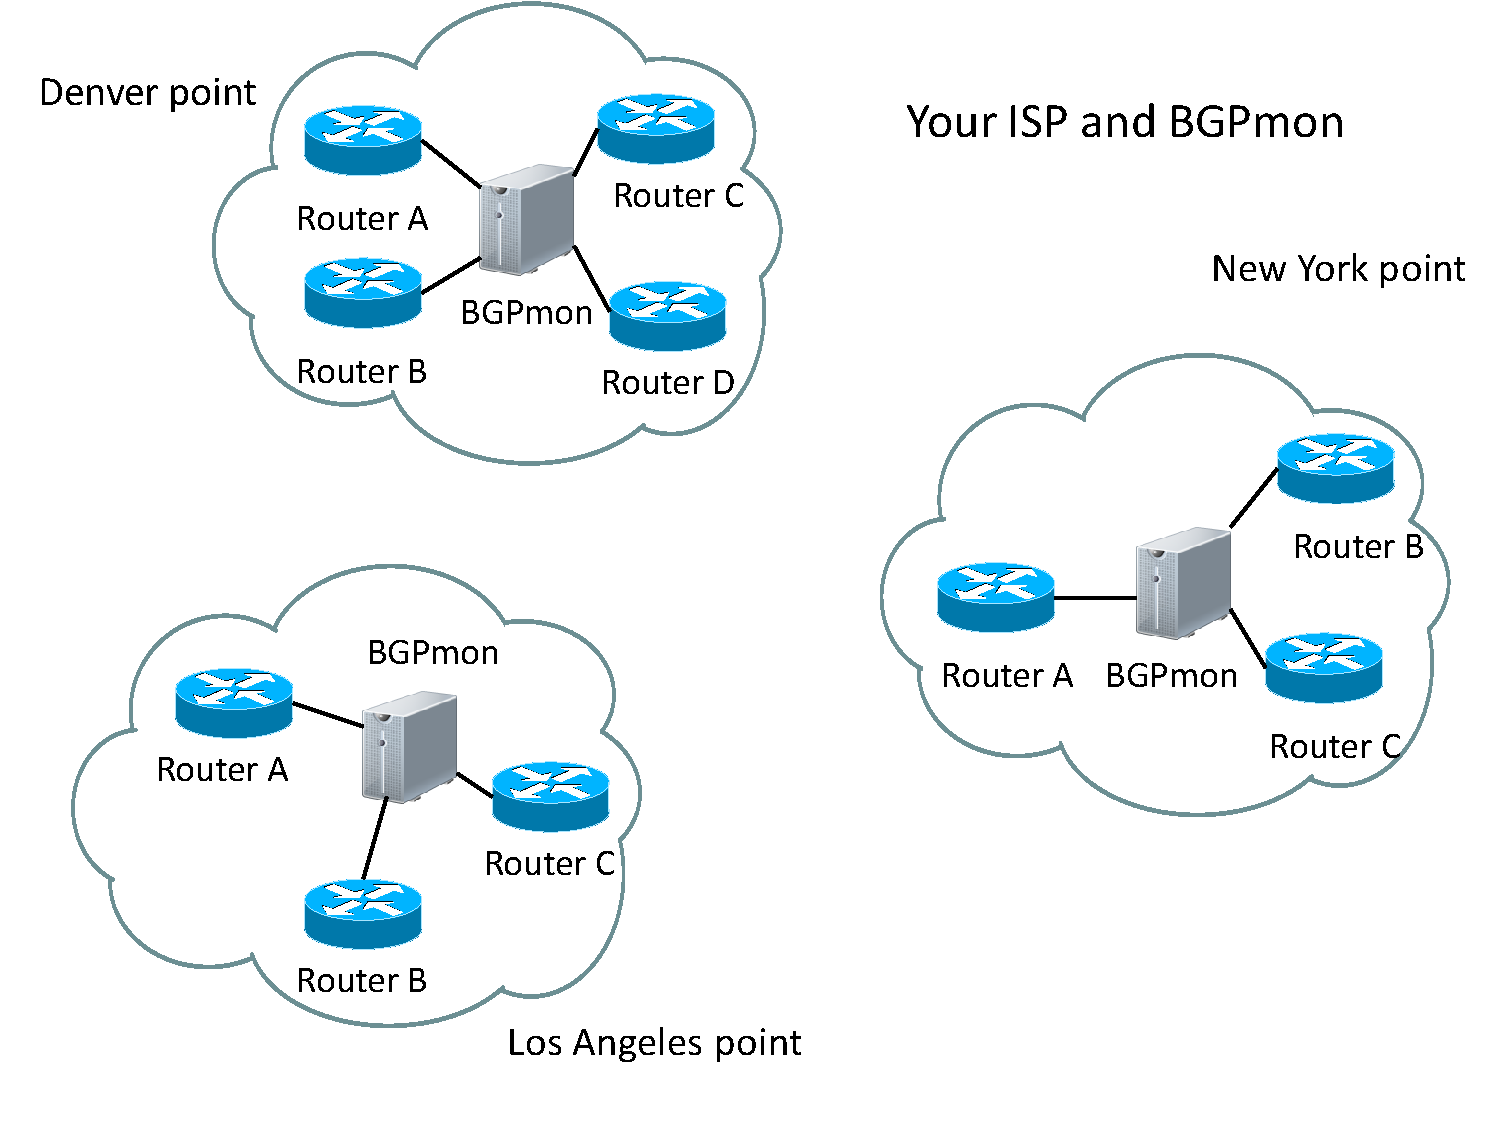
\includegraphics[scale=0.30]{figs/your-isp-and-bgpmon1.pdf}
\caption{BGPmon mesh 1.}
\label{BGPmonmesh1}
\end{figure}




While we have endeavored to design a BGPmon that scales to a large number of peers and clients, we allow BGPmon to scale out through the interconnection of multiple BGPmons. Figure \ref{BGPmonmesh1} shows example of ISP with different router locations around the country. Los Angeles and New York locations has 3 core routers, while Denver location has 4 core routers. All of them runs BGP peering with neighbor peers (not shown in Figure). In this example, we have 3 BGPmon monitors installed in each location. Clients, who's interested in live routing data available at New York location, should subscribe (open a TCP connection) to BGPmon in NY area. 



Moreover, BGPmon is able to to peer with each other monitors and form an overlay network (mesh). Figure \ref{BGPmonmesh2} shows a improved network topology. In our example, we have added two BGPmon core monitors. All BGPmon instances in three locations monitor a unique set of peers and forward their events to BGPmon core monitors.  Each BGPmon core monitors will log the event stream and forward their events to any clients attached. Clients can subscribe to BGPmon core monitors and receive a single stream of routing events happening around the county. 

\begin{figure}
\centering
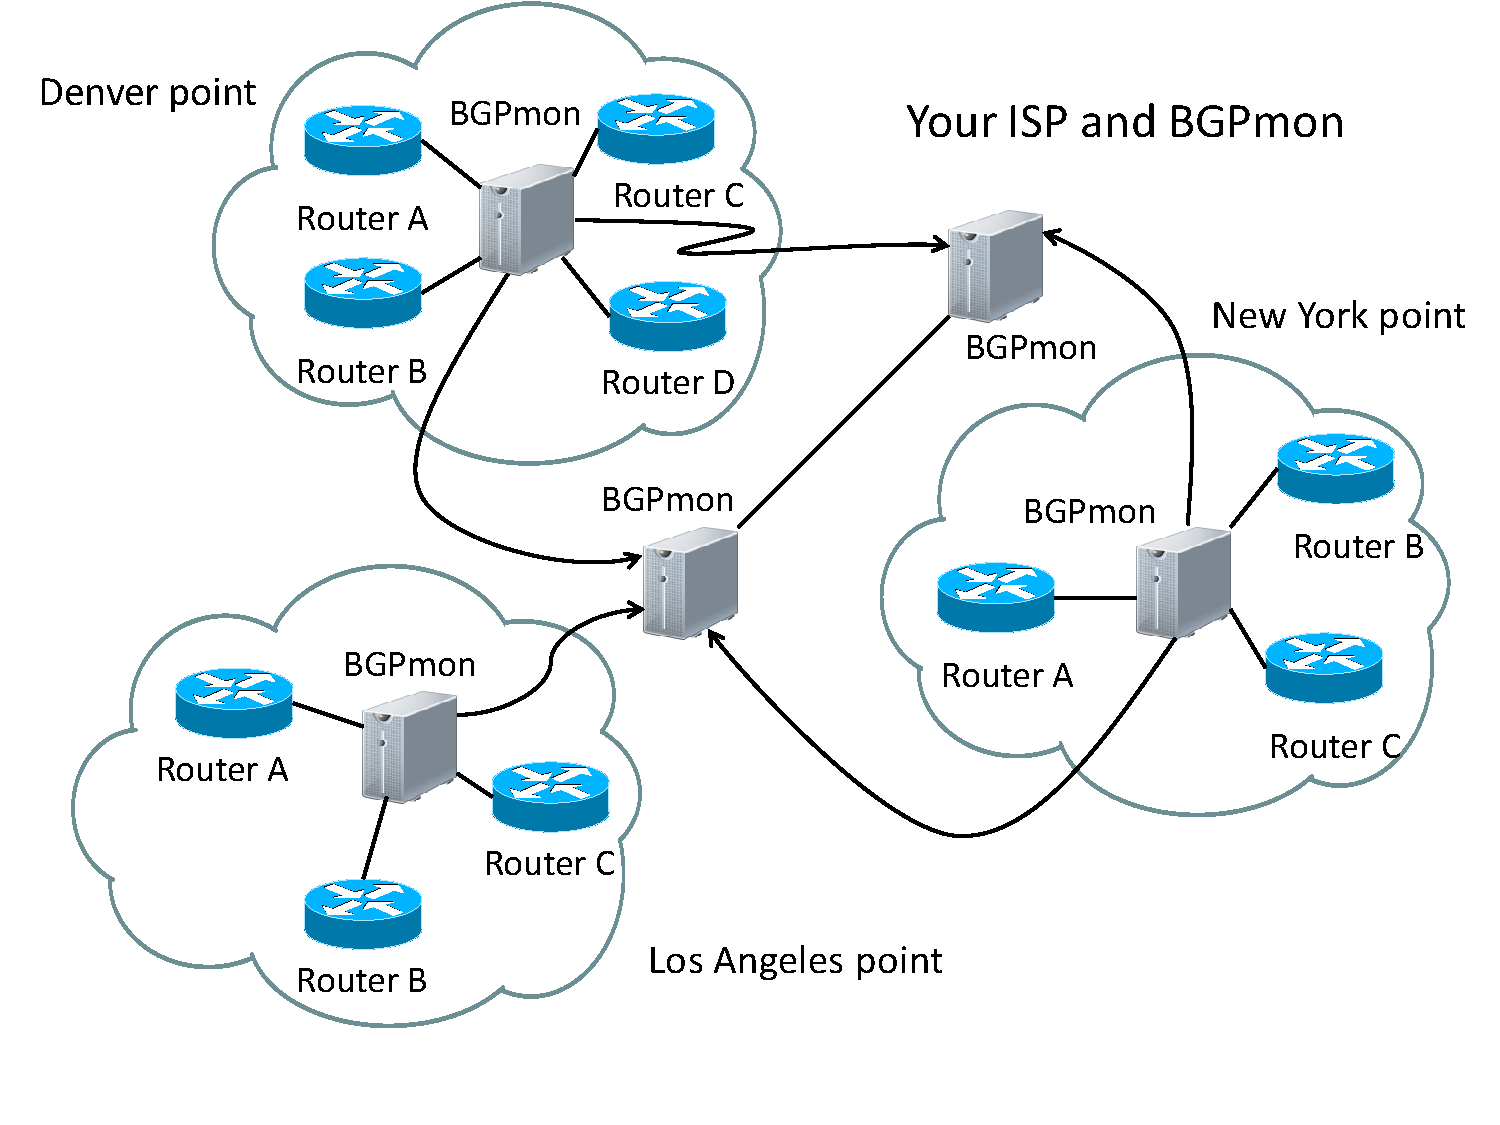
\includegraphics[scale=0.30]{figs/your-isp-and-bgpmon2.pdf}
\caption{BGPmon mesh 2.}
\label{BGPmonmesh2}
\end{figure}

Although BGPmon is able to peer directly with routers, there are exist other Routing Collectors in the Internet (see Section \ref{sec:background}). BGPmon is able to work with these external RCs with a few modifications to the RC software. Currently, Oregon Routeviews\cite{routeviews} collectors provide a routing data to BGPmon. Figure \ref{BGPmonmesh3} shows an example, how, early described ISP network topology, can be modified to receive routing events from RouteViews. This example describes how BGPmon enables scalable real-time monitoring data distribution and create an overlay network (mesh), which provides a single stream without modifying the monitors. 




\begin{figure}
\centering
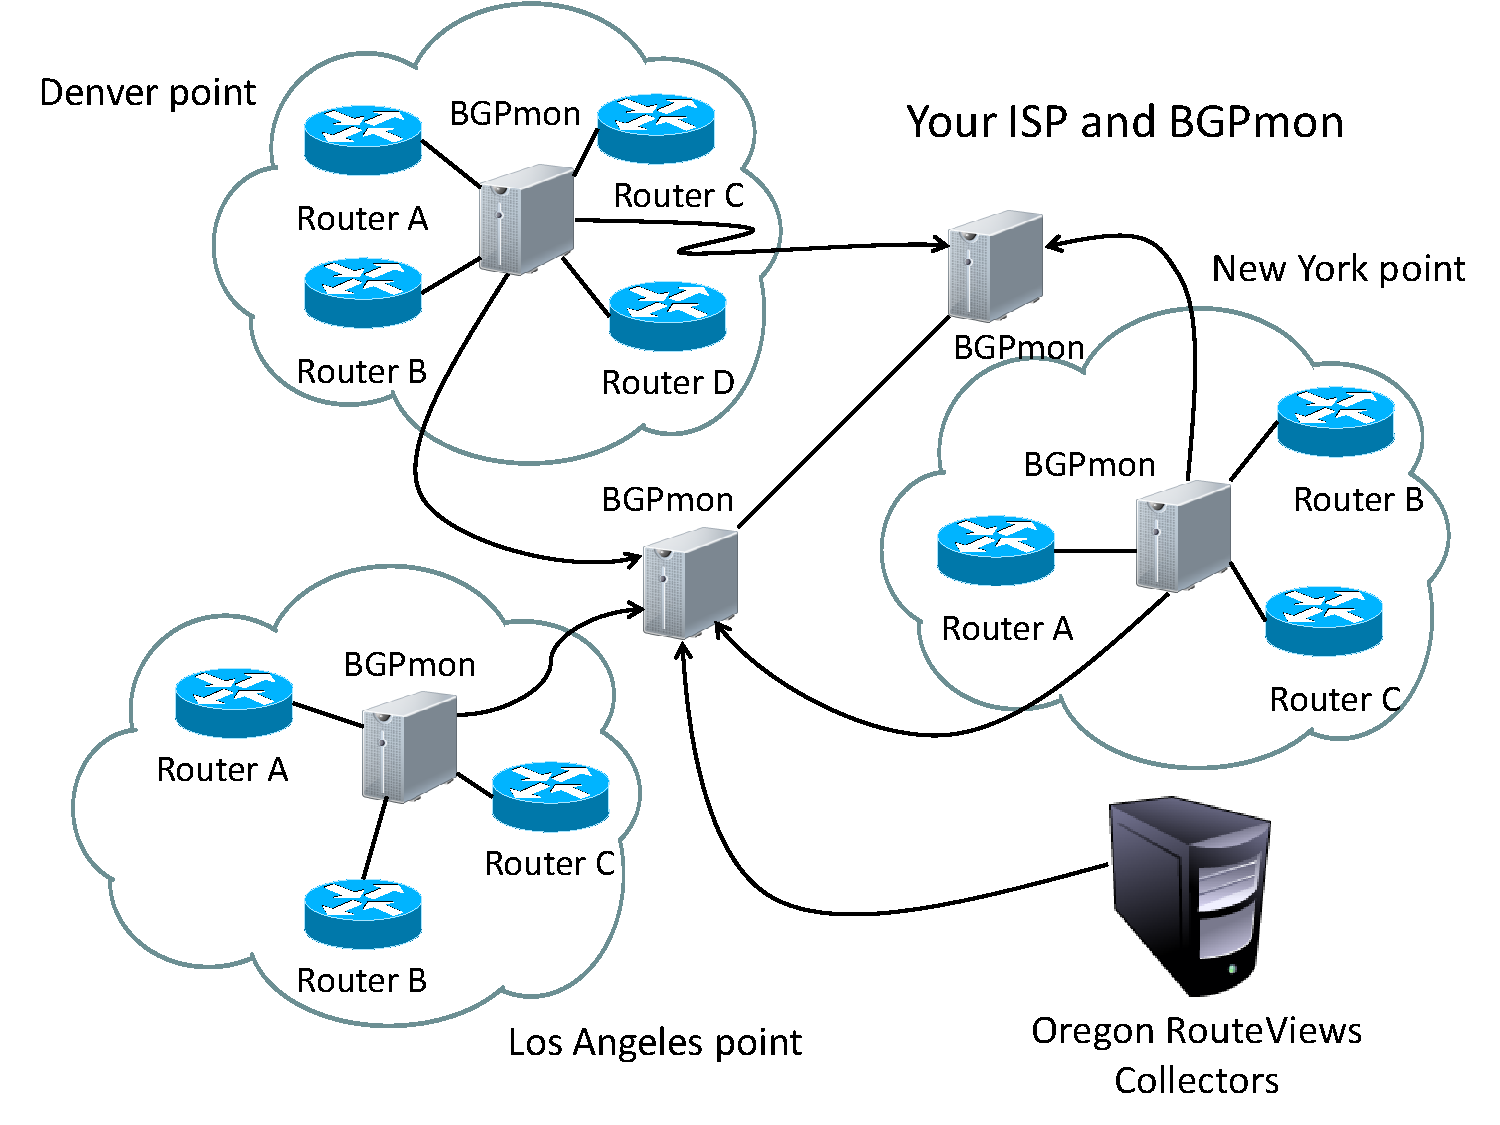
\includegraphics[scale=0.30]{figs/your-isp-and-bgpmon4.pdf}
\caption{BGPmon mesh 3.}
\label{BGPmonmesh3}
\end{figure}